%%%%%%%%%%%%%%%%%%%%%%%%%%%%%%%%%%%%%%%%%%%%%%%%%%%%%%%%%%%%%%%%%%%%%%%%%%%%%%%%%%%%%%%%%%%%%%%%%%%
%%%%%%%%%%%%%%%%%%%%%%%%%%%%%%%%%%%%%%%%%%%%%%%%%%%%%%%%%%%%%%%%%%%%%%%%%%%%%%%%%%%%%%%%%%%%%%%%%%%
\chapter{''Resultados''}

(Por ahora est\'a copiado y pegado un reporte preeliminar sobre los resultados
para tenerlo en cuenta y no olvidarlo; m\'as adelante
escribir\'e una explicaci\'opn adecuada.

Desde el punto de vista formal, se sigue directamente de la descripci\'on del test PSR, y s\'olo
hace falta indicar c\'omo se acomodaron los datos. Desde el punto de vista fisiol\'ogico es m\'as
interesante y extensa la parte que falta.)

Idealmente, esta secci\'on debe ser accesible para personas sin la preparaci\'on fisiol\'ogica
o sin la preparaci\'on matem\'atica.

%%%%%%%%%%%%%%%%%%%%%%%%%%%%%%%%%%%%%%%%%%%%%%%%%%%%%%%%%%%%%%%%%%%%%%%%%%%%%%%%%%%%%%%%%%%%%%%%%%%

\section{Metodolog\'ia}

Primeramente se han considerado los registros polisomnograficos del sujeto [ver parte fisiologica
donde pondre los detalles] en los disntintos
canales por separado. Segun las normas de la AAIC, se separo el registro en \textbf{epocas}
de 30 segundos, obteniendo una GRAN cantidad de series, considerendo que el muestreo se hizo
a 512 Hz --512 puntos por segundo.

Se ha usado el software estad\'istico R junto con el paquete \texttt{fractal} [falta citar].
Como se mencion\'o en la parte matem\'atica, el test PSR fue dise\~nado considerando los
procesos estoc\'asticos a tiempo continuo $\{X(t)\}$, tales que
$E[X(t)]=0$ y $E\left[ X^{2}(t)\right] < \infty$ para todo $t$. La segunda condici\'on
puede considerarse cumplida trivialmente por las caracter\'isticas del modelo, ya que
la energ\'ia dle sistema es claramente finita [quiza deba ser mas explicito el respecto].
La primera condici\'on, en cambio, no tiene porque satisfacerse.

Se forzar\'a a que $E[X(t)]=0$ usando un fitro no-param\'etrico. Debido a que \'unicamente se
espera investigar la estacionaridad, y aun no se ha considerado investigar los motivos o la forma
de la misma, bastar\'a por ahora. Se ha elegido el filtro STL \cite{Coleman87} debido
a que est\'a implementado en R en la librer\'ia base. [en un anexo pongo el c\'odigo
como ejemplo de uso, y quiza otro sobre el STL en si]

Posteriormente, la funcion stationarity del paquete fractal realiza el test PSR
con un resultado como el siguiente

\begin{lstlisting}
Priestley-Subba Rao stationarity Test for datos
-----------------------------------------------
Samples used              : 3072 
Samples available         : 3069 
Sampling interval         : 1 
SDF estimator             : Multitaper 
  Number of (sine) tapers : 5 
  Centered                : TRUE 
  Recentered              : FALSE 
Number of blocks          : 11 
Block size                : 279 
Number of blocks          : 11 
p-value for T             : 0.4130131 
p-value for I+R           : 0.1787949 
p-value for T+I+R         : 0.1801353 
\end{lstlisting}

La prueba sobre estacionariedad se refiere al p-valor sobre el tiempo, el antepen\'ultimo
rengl\'on del resultado; en este ejemplo el p-valor es de 0.1787949 de modo que
la hipotesis de estacionariedad no puede ser rechazada. 

[recordando que deberia poner un anexo sobre que significan los
otros dos valores, y quiza el resto de los datos en pantalla]

El estad\'istico usado es el logaritmo de la potencia del espectro, estimado localmente.
Los puntos en el tiempo y el espacio alejados entre s\'i fueron elegidos de tal forma que
se cubran 'muchos' puntos pero que est\'en lo m\'as alejados entre s\'i como sea posible.
[Los detalles en la implementaci\'on los tengo pero me falta transcribirlos, es un logaritmo
de la cantidad de datos multiplicado por algunas cosas]. Para ver mas detalles vease la parte matematica.

[El espectro puede recuperarse de la prueba, peor no lo hago porque solo
es confiable bajo ciertas hipotesis enn las cuales no he profundizado]

\begin{tabular}{cc}
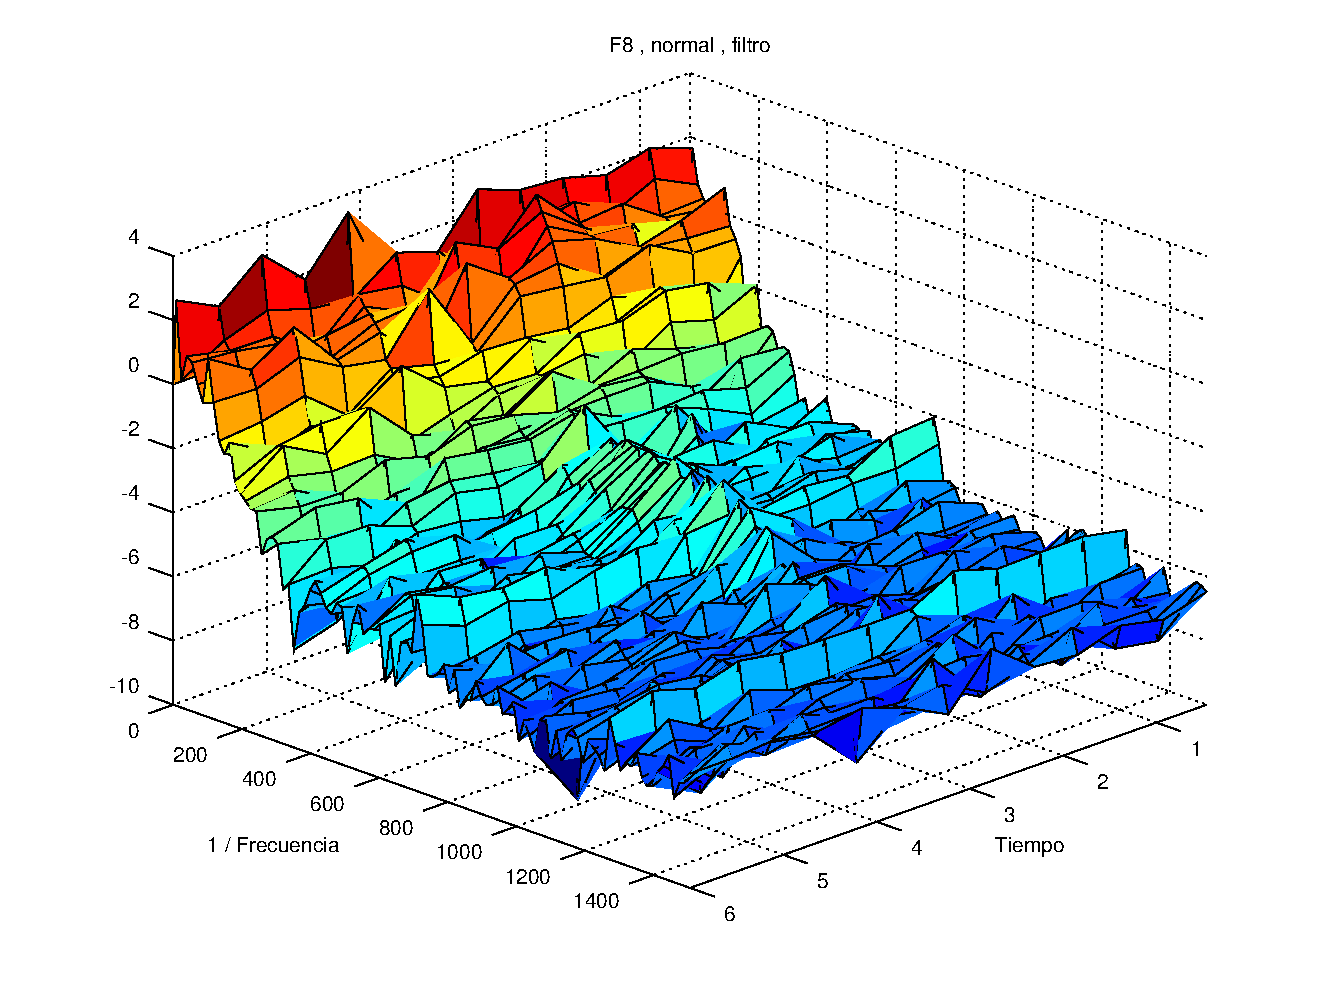
\includegraphics[width=0.5\linewidth]{n8f.pdf} 
&
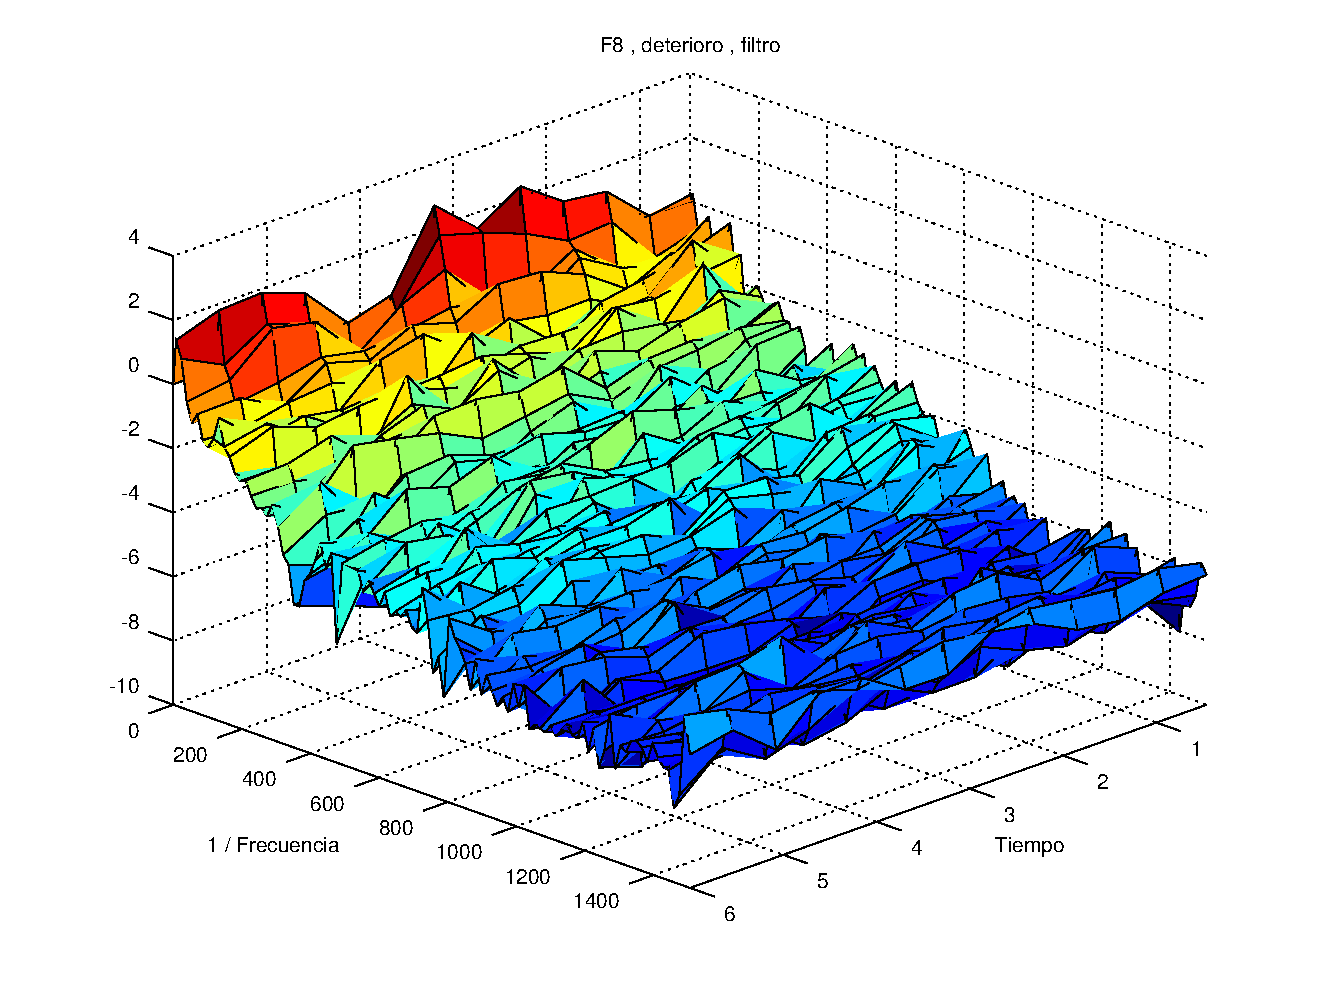
\includegraphics[width=0.5\linewidth]{d8f.pdf} 
\\
\begin{lstlisting}
T      : 0 
I+R    : 5.787895e-09 
T+I+R  : 0 
\end{lstlisting}
&
\begin{lstlisting}
T      : 0.00332259 
I+R    : 0.03502537 
T+I+R  : 0.01598073 
\end{lstlisting}
\end{tabular}

Este test se ha realizado para TODAS las epocas disponibles, pero como el test
es r\'apido s\'olo ha tardado 1 hora por sujeto usando una maquina potente [debo citar
los detalles tecnicos, y la cantidad de puntos procesados. Segun Nason (2012), el test PSR
tiene una velocidad del orden de $N log(N)$, con $N$ la cantidad de puntos procesados, y 
con lo cual es bastante mas rapido que otras pruebas].

%%%%%%%%%%%%%%%%%%%%%%%%%%%%%%%%%%%%%%%%%%%%%%%%%%%%%%%%%%%%%%%%%%%%%%%%%%%%%%%%%%%%%%%%%%%%%%%%%%%

\section{Resultados del test PSR}



\begin{figure}
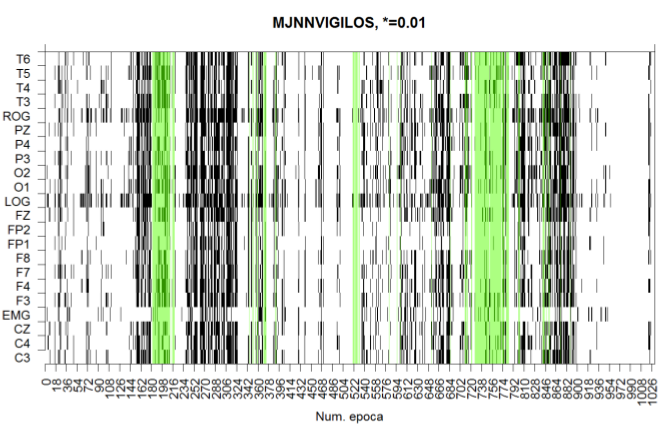
\includegraphics[width=\textwidth]{est01.png} 
\caption{Se muestran los resultados del test PSR de estacionariedad en el sujeto MJNN para las 1032 épocas de sueño en los
22 canales. En el eje horizontal se muestra el número de época, en el eje vertical se muestra al nombre del canal, de
modo que una fila tiene los resultados para un canal durante las diferentes épocas y una columna son los resultados
para todos los canales durante una época dada. En verde se han encerrado las épocas MOR.
Se consideró con un p-valor menor a 0.1 el rechazo de hipótesis nula: el registro en es no-estacionario (blanco),
mientras que el no-rechazo se consideró estacionario (negro).
Total de épocas: 1032 , Épocas MOR: 127}
\end{figure}

\begin{figure}
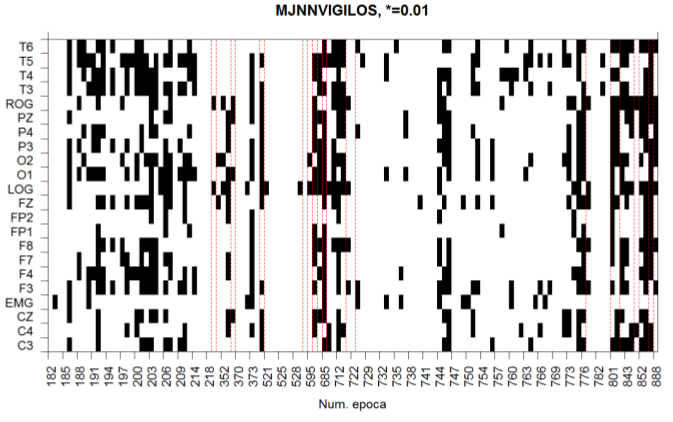
\includegraphics[width=\textwidth]{est02.png} 
\caption{En este gráfico sólo se ilustran épocas MOR. Las líneas punteadas separan bloques continuos.
Total de épocas: 1032 , Épocas MOR: 127}
\end{figure}

%%%%%%%%%%%%%%%%%%%%%%%%%%%%%%%%%%%%%%%%%%%%%%%%%%%%%%%%%%%%%%%%%%%%%%%%%%%%%%%%%%%%%%%%%%%%%%%%%%%
%%%%%%%%%%%%%%%%%%%%%%%%%%%%%%%%%%%%%%%%%%%%%%%%%%%%%%%%%%%%%%%%%%%%%%%%%%%%%%%%%%%%%%%%%%%%%%%%%%%